\subsection{MARCO TEÓRICO}

Esta parte del capítulo expone el contenido teórico necesario para la
realización de este proyecto. Esto incluye información sobre los motores
eléctricos,  análisis de la vibración, las herramientas computacionales, los
sistemas, y el modelado estadístico.

%https://es.wikipedia.org/wiki/Motor_el%C3%A9ctrico


\subsubsection{ Motores eléctricos}

De acuerdo a \Cite{Fraile}, un motor eléctrico es un dispositivo que
transforma energía eléctrica en
energía mecánica mediante la acción de campos magnéticos y están compuestos,
principalmente, por un estator (parte fija) y un rotor (parte móvil).
Existen dos familias principales de motores eléctricos las cuales, a su vez,
se subdividen en \textbf{motores de corriente alterna} como lo son los  motores
de inducción, síncronas, entre otros y los \textbf{motores de corriente continua}
como lo son los motores de escobillas,  sin escobillas, de imán permanente,
entre otros.

El motor mas usado en el sector industrial, es el motor de inducción, debido
principalmente a su bajo costo y al poco mantenimiento que requiere para estar
completamente operativo, esto en particular es debido a su sencillo diseño
en comparación al de otros motores de igual potencia, ya que requiere  menor
número de componentes. Cabe resaltar que el segundo tipo de motor mas usado es
el motor de corriente
continua, debido a que su control, en términos de torque y potencia, es mucho
mas sencillo para ciertos niveles de potencia.

También existen los motores síncronos, cuya construcción es similar a la de un
motor de inducción pero a su vez requiere de una fuente de alimentación externa
para el rotor, lo cual aumenta su costo, además de esto su velocidad es
constante, por lo tanto este tipo de motor es utilizado en aplicaciones
especificas. Como se mencionó anteriormente, existen otros tipos de motores,
pero son usualmente de menor potencia por
lo tanto su utilidad industrial es mucho mas limitada.


\subsubsection*{Rodamientos}

Para que un motor pueda llevar a cabo la transformación de potencia debe rotar.
Esta acción es llevada a cabo por el \textbf{rotor}, el cual esta formado por un
eje que soporta un juego de bobinas envueltas sobre un núcleo magnético. Este
se encuentra suspendido por \textbf{rodamientos}, de forma que el movimiento y
las fuerzas producidas en la interacción entre las bobinas y el núcleo con los
campos magnéticos, producidos por el estator, puedan ser utilizados. Además,
los rodamientos, cuando se encuentran en buenas condiciones, permiten minimizar
el roce entre el eje y soporte, maximizando la transferencia de potencia.

Estos también son conocidos como \textbf{rolineras}, y son un tipo de cojinete,
un elemento mecánico diseñado para reducir la fricción entre un eje y los
elementos conectados al mismo. Existen muchos tipos de rolineras, sin embargo
su estructura se fundamenta en dos anillos concéntricos, algún elemento rotativo
como pueden ser bolas o rodillos, una jaula que se encarga de mantener los
elementos de rodadura separados además de guiados y un lubricante o un sistema
de lubricación.

Dado que son un elemento mecánico el cual es continuamente usado, sufre mucho
desgaste y es el elemento mas propenso a dañarse, según los estudios realizados
por ~\textcite{Kammermann} el 59\% de las fallas son causadas por los rodamientos
y asimismo su principal falla es el desgaste, de igual forma se presentan
otras fallas estructurales. Y por estas razones es fundamental tener bajo continuo
monitoreo este elemento, esto se suele hacer a través de un análisis de vibración.


\subsubsection{Análisis de Vibración}

Como se explica en \Cite{wiki:Vibration}, la vibración, es el  movimiento
periódico de un cuerpo o medio
elástico, alrededor de un punto de equilibrio. En general podemos decir que una
vibración es un caso específico de una oscilación, cuando esta es de origen
mecánico.

Asimismo, se conoce como análisis de vibración, al conjunto de técnicas que permiten
obtener información de un equipo, a partir de sus vibraciones. Es una de las
técnicas más usadas en el mantenimiento predictivo de equipos mecánicos, debido
a que es un proceso poco invasivo y de bajo costo. El análisis de vibración
permite diagnosticar fallas de forma temprana, así como detectar señales
prematuras de desgaste.

Según Girdhar \Cite{Girdhar},  el análisis de vibración nos permite detectar las
siguientes fallas:

\begin{itemize}[noitemsep]

\item Defectos en los engranajes
\item Defectos en los rodamientos
\item Desalineamientos
\item Desbalances
\item Ejes torcidos
\item Excentricidad
\item Fallas eléctricas
\item Fuerzas hidráulicas o aerodinámicas
\item Mala sujeción en las piezas
\item Problemas en las correas de transmisión
\item Problemas de lubricación
\item Resonancia
\item Rozamientos en el rotor
\end{itemize}


\subsubsection*{Adquisición de datos}

Para realizar cualquier tipo de análisis, primero se deben adquirir datos y,
por regla general, mientras mas datos se tengan y mas precisas sean las
mediciones, mejores serán los estudios que se pueden realizar.


La adquisición de datos, según \cite{adquisiciondatos}, es el proceso de
realizar mediciones de fenómenos físicos
y registrarlos, en algún formato específico, para analizarlos posteriormente.
Cabe resaltar que en algunos casos es necesario hacer un acondicionamiento de
la señal, esto
implica modificarla controladamente al reducir o aumentar su amplitud además de
sumarle un nivel offset, voltaje continuo, para que cumpla requisitos mínimos
y pueda ser procesada por los siguientes circuitos.

Al momento de la adquisición de datos, se toman medidas de una señal analógica
la cual se convertirá al pasar por una serie de etapas y dispositivos en una
señal digital y se guardará en un formato deseado y en una unidad de
almacenamiento masivo (ROM, flash, etc).
El primer paso en la toma de  datos comienza con el sensor, que es un
dispositivo el cual transforma la unidad física de interés, en una señal que
pueda ser procesada con mayor facilidad, luego esta se adecuará mediante un
circuito especializado a las características y requerimientos del sistema,
luego será procesada por un convertidor Analógico-Digital, el cual se encarga de
muestrear, retener y procesar la señal y, de esta forma, obtener una versión
digital de la misma, la cual se procesará o guardará mediante un software desde
una computadora.

En el caso de las vibraciones, los sensores mas usados son los
acelerómetros.  Esto se debe principalmente a que tienen mayor ancho de banda
que los sensores de posición y los de velocidad, lo que les permite detectar
vibraciones de mayor frecuencia. Adicionalmente, dado que las vibraciones en los
rodamientos, por naturaleza, son de alta frecuencia y, como se mencionó anteriormente,
estos son componentes críticos en los motores eléctricos.
Estas características hacen al acelerómetro el sensor mas utilizado para las
mediciones de vibración en motores eléctrico. Sin embargo,
en casos mas especializados, como podría ser el análisis de vibración
de maquinaria de larga envergadura, son también usados los otros tipos de
sensores ya que sus características pueden facilitar el estudio.


\subsubsection{Acelerómetros}

Un acelerómetro es un dispositivo capaz de medir aceleración, no es
necesariamente la misma que la aceleración de coordenadas (cambio de la velocidad de
un elemento en el espacio), sino que es la correlación asociada con el fenómeno
de peso experimentado por una masa de prueba que se
encuentra en el marco de referencia del dispositivo.  Funciona mediante
la utilización de la segunda ley de Newton, \textbf{la fuerza resultante
ejercida sobre un cuerpo es proporcional a su masa por su aceleración}. Los
acelerómetros por lo general cuentan con una masa de prueba (también conocida
como masa sísmica), alguna especie de resorte y un marco de soporte que, a su
vez, puede funcionar como amortiguador. Debido a esto, los acelerómetros se
pueden modelar matemáticamente como un sistema lineal de segundo orden,
por lo que su respuesta en frecuencia posee un pico de resonancia.


\subsubsection*{Tipos de acelerómetros}

\begin{itemize}
    \item  Acelerómetros Capacitivos:

        Los acelerómetros capacitivos son uno de los modelos mas sencillos
        capaces de medir
        aceleración, además de ser fácilmente utilizables y reproducibles en masa.
        Funcionan mediante una masa sísmica, dado que, al  experimentar una fuerza
        se desplaza con una aceleración proporcional a la fuerza aplicada.
        Si a la masa se le agregan unos resortes unidos a una carcasa, los resortes
        ejercerán una fuerza proporcional al desplazamiento de la masa generando un
        desplazamiento fácilmente medible.

        Este fenómeno se produce ya que estos efectos en conjunto al
        amortiguamiento producen un sistema lineal de
        segundo orden, este sistema matemático genera una salida en desplazamiento
        al aplicarse como entrada una fuerza
         Finalmente, al conectarse un sensor de desplazamiento, se observa
        la aceleración a la que esta sometido el instrumento.
        El sensor de desplazamiento mas
        popular para este tipo de medidores es el capacitivo.

        En su mayoría los acelerómetros capacitivos vienen como dispositivos
        microelectromecánicos, \textbf{mems} por sus siglas en inglés, que son
        dispositivos
        fabricados con técnicas similares a las de fabricación de circuitos
        integrados, a su vez poseen componentes mecánicos microscópicos. Son los
        acelerómetros mas populares en aplicaciones no industriales, sin embargo,
        en aplicaciones de bajo consumo, bajo coste o cuando las frecuencias con
        las que se trabajan no son tan altas, pueden ser usados a niveles
        industriales, ya que poseen múltiples ventajas como:

        \begin{itemize}[noitemsep]
            \item No requieren adecuación de la señal.
            \item Pueden comunicarse directamente con un microcontrolador.
            \item Su precio es económico.
            \item Son compactos.
        \end{itemize}


    \item  Acelerómetros piezoresistivos:

        Son, después de los acelerómetros piezoeléctricos, los mas usados a nivel
        industrial. Su funcionamiento es similar al de los acelerómetros
        capacitivos, ante una aceleración de entrada se produce un desplazamiento
        de salida, mas en este caso, estos están constituidos por una o varias
        galgas extensiométricas, una masa de prueba y unos resortes de soporte.
        La galga sujeta a la masa sísmica y, al esta recibir una fuerza, produce
        un desplazamiento proporcional a la fuerza aplicada, lo que deforma a
        su vez la galga extensiométrica lo cual se traduce como un
        cambio de resistencia en el sensor. La ventaja de los acelerómetros
        piezoresistivos es que pueden medir valores de voltaje DC lo que los
        hace útil en el estudio de impactos, son también usados en el
        análisis de vibración en el rango de mediana frecuencia.


    \item Acelerómetros piezoeléctricos:

        Son el acelerómetro mas usado en aplicaciones industriales ya que
        poseen características como:

        \begin{itemize}[noitemsep]
            \item Alto rango dinámico.
            \item Bajos niveles de ruido.
            \item Alta linealidad.
            \item Alto ancho de banda.
            \item Poco desgaste, ya que no poseen partes móviles.
        \end{itemize}


        Su construcción es bastante sencilla, se tiene disco de un cristal
        piezoeléctrico unido por dos terminales circulares, de forma similar a
        la de un condensador, y justo encima tienen una masa de prueba.
        Al experimentar una fuerza el cristal se deforma lo que produce una
        diferencia de carga y un voltaje proporcional a la fuerza aplicada.
        Como la aceleración de la masa de prueba es también proporcional a la
        fuerza aplicada, la aceleración del acelerómetro será entonces
        directamente proporcional al voltaje y la carga producida en el cristal.

\end{itemize}


\subsubsection{Procesamiento de señales}

Después de ser almacenada la información, debe ser estudiada, procesada, para lo
cual se utilizan una serie de herramientas, técnicas o software especializados
a cada necesidad. Este estudio se puede categorizar en dos ramas principales:

\begin{itemize}
    \item Dominio del tiempo, según \cite{wiki:DominioTiempo}, es un término
        utilizado para describir el análisis
        de funciones matemáticas o señales con respecto al tiempo, la sucesión
        de estados que atraviesa la señal de forma natural. Los estudios mas
        comunes son en  \textbf{tiempo continuo} y en \textbf{tiempo discreto}.

    \item Dominio de la frecuencia, según \cite{wiki:DominioFrecuencia}, es un
        término utilizado para describir el análisis
        de funciones matemáticas, señales o movimientos periódicos respecto a
        su frecuencia, número de veces que sucede un evento en un periodo.
        Utilizan transformadas para llevar las funciones o señales del dominio
        del tiempo, base, al dominio de la frecuencia, deseado, la mas famosa es
        la \textbf{transformada de Fourier}.
\end{itemize}


Gráficamente se suele entender el \textbf{dominio temporal} como la evolución
de una señal con respecto al tiempo, es decir su evolución natural, por otro
lado el \textbf{dominio frecuencial} muestra los componentes de la señal según
la frecuencia en la que oscilan dentro de un rango determinado.
En la figura \ref{Dominios} se observan ejemplos gráficos de señales en ambos
dominios.

	\begin{figure}[htb]
		\centering
        \caption{ Diagrama de los dominios temporal y frecuencial}
        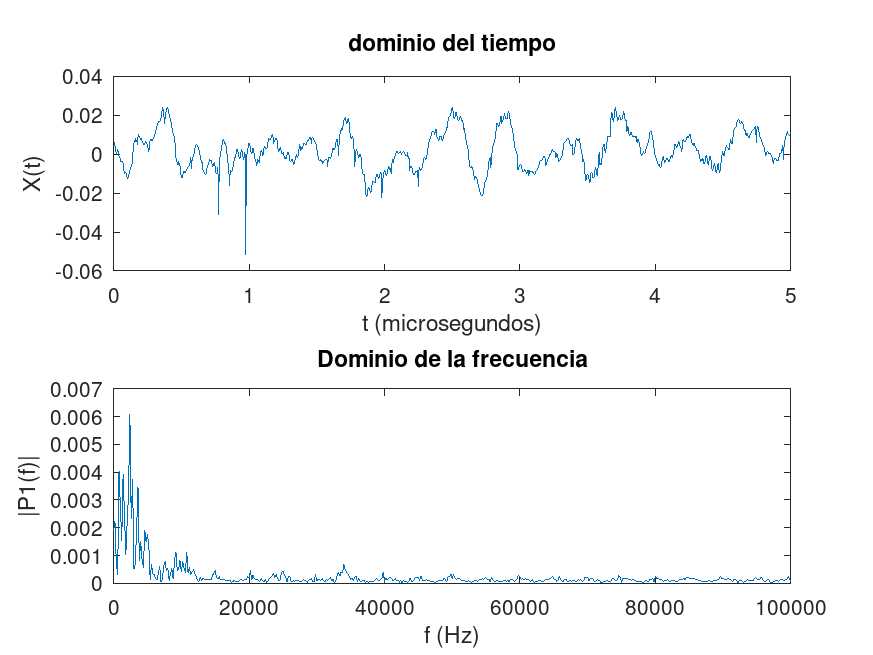
\includegraphics[width=\linewidth]{Dominios.png}
        Realizada con el Software Octave a partir de los datos de.
                \Cite{HUANG20181745}
        \label{Dominios}

	\end{figure}


El análisis en frecuencia suele ser mas utilizado debido a que
la mayoría de las fallas poseen frecuencias características y, dado que en  el
análisis de frecuencia se descompone en frecuencias la señal, se facilita la
detección de fallas características, así mismo, la amplitud de la frecuencia es
directamente proporcional al nivel de la falla. Por lo tanto se obtiene un
espectro amplio del estado de la pieza.
Cabe resaltar que cuando las frecuencias son bajas o muy cercanas entre si,
se dificulta determinar e identificar alguna falla, suele suceder cuando se
estudia una falla o evento con frecuencia muy baja o muy cercana a la frecuencia
natural de la señal o elemento medido. En estos casos es mejor
usar un análisis en el dominio del tiempo que  facilita la
detección de las fallas.



\subsubsection{Herramienta Computacional}


Según \Cite{Herramienta}, una herramienta computacional puede ser definida  como
cualquier software,
sistema de integración, análisis o almacenamiento que  ayuda a los científicos
o usuarios a solucionar un problema específico en una determinada rama. Pueden
variar desde sistemas complejos como compiladores, algoritmos
e incluso sistemas operativos hasta herramientas como hojas de cálculos, sistemas
de oficina o medios de comunicación. Funcionan mediante la implementación de
técnicas y protocolos para solucionar problemas de forma iterativa o con una
secuencia de pasos concreta.

Siguiendo este orden de ideas, una gran cantidad de estas herramientas son
encontradas en la librería de información mas grande del mundo, el Internet.
Todas comparten la peculiaridad de que son un \textbf{sistema} y,  por ende, pueden
ser accedidas con facilidad desde cualquier punto con un dispositivo capaz de
tener conexión a Internet y un navegador. Esta facilidad se debe a que un
\textbf{servidor} se encarga de hacer el procesamiento de la información y envía
el resultado con un formato específico, típicamente son  JSON, por \comillas{notación de
objeto de JavaScrip} el cual es un formato de texto sencillo para el intercambio de
datos, este se renderiza (proceso para generar una representación gráfica por
medio de programas informáticos) en una pagina Web.

\subsubsection{Sistema Web}

Los sistemas Web, de acuerdo a \cite{SistWeb1} y \cite{wiki:systemWeb}, o
también conocidos como aplicaciones Web son sistemas que
utilizan la tecnología Web y el Internet o Intranet para transmitir la
información y los
servicios a usuarios o otros sistemas/aplicaciones. Estos sistemas utilizan los
principios del hipertexto para renderizar la información en cualquier
navegador o \textbf{pagina Web} y el poder de los \textbf{servidores} para
almacenar y procesar la información. Por estas características son independientes
de cualquier plataforma o sistema operativo, además de  no requerir ningún
proceso de instalación, facilitando de esta forma el acceso, la gestión y la
rapidez de obtención de información.



\subsubsection*{Página Web}
Una página Web es un documento accesible desde cualquier navegador con acceso
a Internet que puede incluir audio, vídeo, texto y sus diferentes
combinaciones.
Funciona al usar el protocolo HTTP, conocido usualmente como la Web, y una
estructura de hipertexto la cual permite redirigir, enlazar y estructurar el
contenido y lo hace fácilmente accesible desde un navegador Web.

Funciona gracias al protocolo HTTP, \comillas{Hypertext Transfer Protocol},
el cual es la base de cualquier intercambio de datos en la Web y un protocolo
de estructura cliente-servidor, esto implica que una petición de datos es
iniciada por el elemento que recibirá los datos (el cliente), normalmente un
navegador Web, y es cubierta por el elemento que envía los datos (el servidor).
Este protocolo comenzó siendo estático y dirigido usualmente a la transmisión de
texto pero se fue convirtiendo en mas que eso y en la actualidad permite la
transferencia de documentos de todo tipo, scripts, vídeos, entre otros; a tal
punto que es fácilmente categorizado como el protocolo mas usado en todo el
mundo, siendo incluso utilizado como sinónimo de Internet cuando es solo una
parte de él.

Debido a la invención de tecnologías como javascrit y AJAX hoy en día es
posible tener aplicaciones Web, que son programas junto a una interfaz gráfica,
que permite comunicarse con servidores que realizan la mayor parte del trabajo.
 Es posible el desarrollo de aplicaciones complejas que funcionen desde la
comodidad de dispositivos móviles. La Web permite, por tanto, facilidad a la hora
de transmitir información así como el poder acceder a cualquier contenido desde
cualquier dispositivo en cualquier momento.

La Web suele ser el método de acceso de muchas tecnologías y, si bien en la actualidad
el desarrollo Web usa el mismo estándar de tecnologías, el lado del servidor
contempla una variedad mucho mas amplia, dado que cualquier aplicación que
pueda correr en un ordenador puede ser conectada a una interfaz Web. Teniendo
como limitante principal la latencia,  tiempo que tarda la información en viajar,
una interfaz Web es, para un usuario promedio, una solución cómoda y
accesible la cual  permite incluso  mayor comodidad y facilidad de acceso.


\subsubsection*{Servidor}

Un servidor Web, como lo define \Cite{servidor},  es un ordenador de propósito
específico que permite la
transición de datos a uno o múltiples clientes Web. Para esto, el dispositivo
debe de estar configurado para escuchar las solicitudes de los clientes en un
entorno red. Esto se logra mediante una aplicación externa o el uso de un
sistema operativo dedicado; almacena los archivos
necesarios para el procesamiento de información y los datos necesarios para
mostrarla, además, se encarga de distribuirla al usuario final.

Los servidores se suelen clasificar según su función y es común que cumplan mas
de una función, o se encuentren mas de un tipo en una red. Algunos de estos son
servidores de archivos, impresión, aplicaciones, DNS, \textbf{Web}, entre otros.
Actualmente, los servidores Web son los mas abundantes en el mercado
y se caracterizan por alojar la información y los datos de los usuarios a través
de Internet o Intranet. Estos responden a las solicitudes de paginas Web u otros
servidores basados en esta tecnología.


\subsubsection{Modelo estadístico}

Un modelo estadístico, de acuerdo a \cite{modeloIBM}, es una representación
matemática que permite, mediante
ecuaciones, codificar información extraída de los datos y, de esta forma,
predecir el comportamiento de un sistema ante situaciones dadas. Funcionan
mediante  variables aleatorias, una o mas variables de las cuales no
se tiene completa certeza de su valor o provienen de algún evento aleatorio.

Un modelo estadístico permite inferir ciertas características de un evento,
como qué tan probable es tal evento y cómo se distribuyen los valores de la
variable. Además se suele usar como primer paso en generar un modelo mas
preciso o para la obtención de información cuando no se tiene suficiente,
es difícil su acceso o la naturaleza del
sistema es extremadamente compleja y dicha tarea es simplemente imposible.
